\epigraph{A supercomputer is a device for turning compute-bound problems into I/O-bound problems}{Ken Batcher}

\minitoc

% to add
% 0. limits of laptops/PCs/workstations/clusters/supercomputers
% 1. size of problems and data requirements
% 2. estimates for some calculations
% 3. Moore's law
% 3.1 charts (top500.org)
% 3.2 history
% 3.3 variants (cpu, gpu, hard drive, memory)
% 3.4 trends
% 3.5 outlook

% https://en.wikipedia.org/wiki/Moore%27s_law
% https://www.intel.com/content/www/us/en/silicon-innovations/moores-law-technology.html
% https://www.nextplatform.com/2017/03/22/memory-logic-post-moores-law-world/
% https://www.afr.com/chanticleer/technology-disruption-to-accelerate-as-moores-law-dies-20180719-h12wrv
% google "the death of Moore's law"
% chip manufacturers (Global Foundaries, TSMC, Samsung, clients: Intel, Apple, AMD, NVIDIA)
% https://www.youtube.com/watch?time_continue=164&v=vK-geBYygXo

% What is HPC
% https://insidehpc.com/hpc-basic-training/what-is-hpc/

In this lecture we give an overview of High Performance Computing (HPC). Here are some definitions of HPC gathered using google:

\begin{itemize}
    \item[] From \href{https://insidehpc.com/hpc-basic-training/what-is-hpc/}{InsideHPC.com}: '
    
    ``\emph{HPC most generally refers to the practice of aggregating computing power in a way that delivers much higher performance than one could get out of a typical desktop computer or workstation in order to solve large problems in science, engineering, or business.}''
    \item[] From \href{https://www.netapp.com/us/info/what-is-high-performance-computing.aspx}{NetAPP.com}: 
    
    ``\emph{HPC is the ability to process data and perform complex calculations at high speeds. To put it into perspective, a laptop or desktop with a 3 GHz processor can perform around 3 billion calculations per second. While that is much faster than any human can achieve, it pales in comparison to HPC solutions that can perform quadrillions of calculations per second.}''
    \item[] The \href{https://en.wikipedia.org/wiki/Supercomputer}{Wikipedia HPC page} includes a lot of information but does not actually define HPC.
    \item[] From  \href{https://www.techopedia.com/definition/4595/high-performance-computing-hpc}{Techpedia.com}: 
    
    ``\emph{HPC is the use of super computers and parallel processing techniques for solving complex computational problems. HPC technology focuses on developing parallel processing algorithms and systems by incorporating both administration and parallel computational techniques.}
    
    \emph{High-performance computing is typically used for solving advanced problems and performing research activities through computer modeling, simulation and analysis. HPC systems have the ability to deliver sustained performance through the concurrent use of computing resources.}''
    \item[] From \href{https://www.nics.utk.edu/computing-resources/what-is-hpc}{National Insititute for Comptutational Science @U. Tennessee, Knoxville}:  
    
    ``\emph{HPC, is the application of ``supercomputers'' to computational problems that are either too large for standard computers or would take too long.}''
\end{itemize}
% https://hpc-wiki.info/hpc/Shell
A recurrent theme in these descriptions of HPC is using parallel computing techniques on large scale systems (like clusters or super-computers) to exceed the performance and/or capacity of a typical laptop or desktop computer. In reality there is more to HPC than merely running large calculations on large scale clusters. In the following sections we break down different aspects of HPC.

\section{Calculations with large data requirements}

When you purchased your laptop and chose the model with 8GB memory\footnote{See Section \ref{dataSizes.sec} for the definition of gigabytes (GB).} you probably didn't think about the intrinsic limitations of that choice. With 8GB of random access memory (RAM) you can keep at most  one billion double precision variables in system memory at one time \footnote{You can conceivably perform calculations with more than a billion doubles on your laptop, if you are patient and are ok using the slower hard drive or solid state drive usually used for storing files to store your data during the calculation.} 

What do you do if you want to work on problems that need more than a billion doubles, for instance when you are solving a problem with tens of billions of degrees of freedom ? You may be able to install extra RAM, or buy a computer with more RAM at some considerable cost of course. Indeed some workstations are equipped with a terabyte of RAM, raising the capacity to a hundred billion doubles simultaneously in memory. Unfortunately the time it takes to process a problem typically  increases with the problem size and with that extra memory we would be wise to upgrade the central processing unit (CPU). But what should we do if our target problem requires many terabytes of data ?

\section{Calculations that take a long time}

While some calculations may require large amounts of data, other calculations may conversely have very small memory footprints yet take an inordinately long time\footnote{The word inordinately derives from the Latin root verb ``ordinare'' which means to arrange. Entertainingly this root verb is shared by the French word for computer ``ordinateur''. Furthermore, the French word ``ordinateur'' \href{https://blogs.transparent.com/french/the-origin-of-lordinateur-computers-in-french/}{was introduced into the language by IBM in the 1950s} and it became a commonly used word before they could trademark it.} 

Consider for instance the task of finding all the prime numbers up to a given large number $N$. One brute force approach with almost no memory requirements is to test if each number is divisible by all the integers less than its square root. Admittedly this is a very inefficient way of finding the primes but let's suppose for the sake of this example that in some parallel universe  \href{https://en.wikipedia.org/wiki/Sieve_of_Eratosthenes}{Eratosthenes} did not invent the prime sieve and mathematicians had paid no attention to primes and thus brute force calculation is the only known strategy. In that universe we would be obliged to perform (pessimistically) $\mathcal{O}(N^{3/2})$ divisions to find the primes up to $N$. Now let's imagine that in this alternative universe although the Mathematicians had been asleep at the wheel, computer engineering was just as advanced. The alt world computer scientists would observe that each integer can be tested independently for primality independently of all the other integers. Thus if we split the primality tests amongst $P$ processors then it should be possible to reduce the calculation time from $\mathcal{O}(N^{3/2})$ to $\mathcal{O}(N^{3/2}/P)$ which will make it possible to compute the primes to larger $N$ for a fixed wall clock time. However, that alternative universe will still come to an end before the calculations terminate for sufficiently large $N$.

Fortunately in our universe the Sieve of Eratosthenes was discovered early and improved on over time. \href{https://en.wikipedia.org/wiki/Sieve_of_Eratosthenes}{It and more recent variants} are significantly more efficient than brute force testing making the above discussion moot. Furthermore there are many \href{https://en.wikipedia.org/wiki/Primality_test}{alternative ways for testing for primality} if that is your goal.

\section{Moore transistors, Moore compute}

In 1965 Gordon Moore of Intel predicted a decade of exponential increase\footnote{See the first graph of \cite{moore1965cramming} for a honest to goodness  exponential growth chart that actually came to pass. This is one of only a few true exponentially varying processes that has continued for forty years.} in economically viable processor capability improvements. 

\begin{figure}[htbp!]
    \centering
    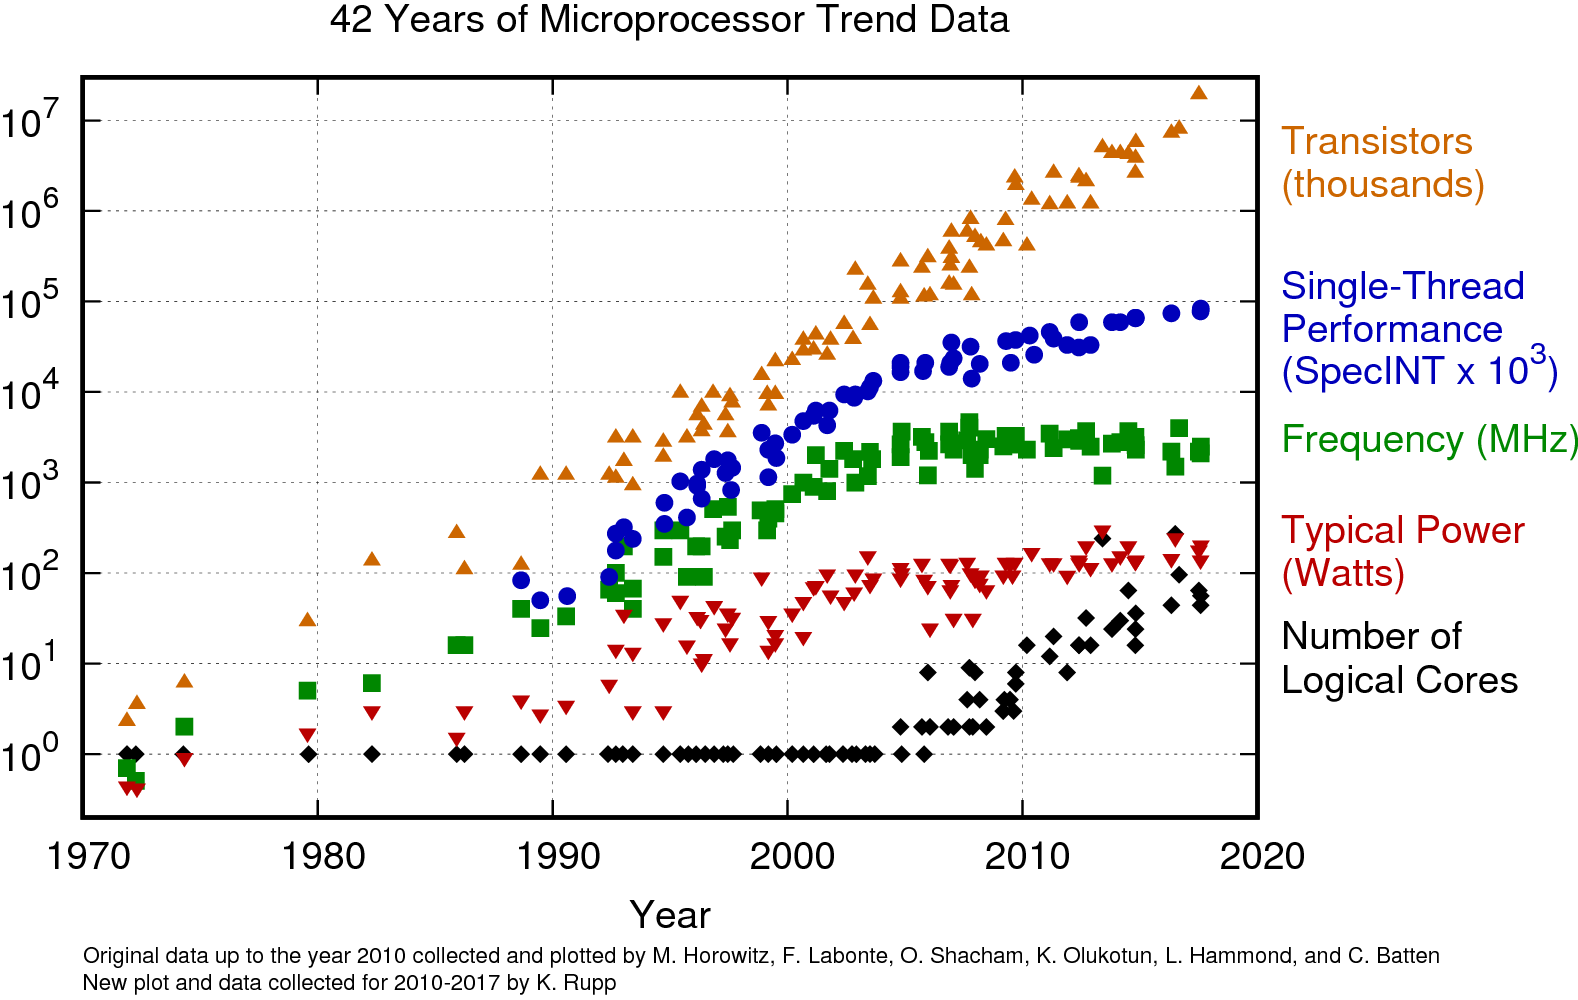
\includegraphics[width=0.95\textwidth]{figures/L13/42-years-processor-trend.png}
    \caption{Trends in processor design. Image sourced from \href{https://www.karlrupp.net/2018/02/42-years-of-microprocessor-trend-data/}{Karl Rupp}. Source data is available on GitHub \href{data: https://github.com/karlrupp/microprocessor-trend-data}{here}.}
    \label{mooresLaw.fig}
\end{figure}


The increase in processor complexity and efficiency coupled with increased clock frequency continued unabated for forty years (from 1965 to 2005) until thermal considerations finally limited clock frequency for monolithic ``serial'' processors. In Figure \ref{mooresLaw.fig} we show the growth in single core processing power. Notice the leveling off in performance in 2005. In particular the single thread performance benchmark shows little recent increase and the manufacture spec core frequency has declined slightly over time. The ``Typical Power'' requirement of the CPU is the key factor that limits the frequency and thread performance. To be precise dissipating the heat generated by the processor at higher clock frequencies is the major hurdle that forces manufacturers to curtail ever increasing the CPU clock frequency. This is because the power consumption of the CPU varies nonlinearly with clock frequency, some analyses show a cubic relationship between clock frequency and power consumption of the CPU !

After 2005 the bulk of CPU performance improvements have resulted from increasing the number of separate processor cores in each CPU. Nowadays the task of exploiting multiple cores on a single CPU rests with the programmer. In the following lectures we will introduce the predominant programming models used to divvy work up amongst multiple cores. We will focus initially in particular on the Open Multi-Processing (OpenMP) approach to parallel programming. Writing an OpenMP program entails annotating a regular Fortran, C, or C++ program with special compiler directives that instruct the compiler to split work amongst multiple cores. 

A carefully crafted OpenMP implementation of a calculation that is particularly well suited to execution by multiple threads on multiple cores of a modern CPU can attain over an order of magnitude performance improvements over the same program running in serial on a single CPU core. However the key phrases here are ``carefully crafted'' and ``particularly well suited to execution by multiple threasd''. This is by no means true of all calculations and should serve as a reality check before you get too excited.

The brutal truth is that a modern Intel CPU with over two dozen processor cores can deliver less than 5\% of its potential performance when running a serial code. In fact a serial code that does not take advantage of the single instruction multiple data (SIMD) vector floating point units (FPU) built into each CPU core and only executes scalar arithmetic operation at time, i.e. one floating point operation per clock cycle, will achieve less that 1\% of the theoretical peak of the CPU floating performance. Imagine that you only score 1\% in every homework assignment, not a great achievement, but so far in your academic careers it is very likely that any code you have written has achieved that very modest level of achievement.

\section{Scaling up}

The US Department of Energy (DOE) is tasked with nuclear stockpile management and general computational modeling for energy applications. Modeling for energy related applications inevitably involves evaluating computational models quite often involving complicated dynamical systems with potentially trillions of state variables. For example modeling turbulence in fuel injectors, heat exchange processes and neutronics in nuclear reactors, efficient energy capture in wind farms, design and analysis of nanoscale manufacturing processes, urban environmental heating, and many more energy related problems. The DOE has been a national and worldwide leader in building increasingly powerful supercomputers and software to deploy on these systems to address these large scale modeling problems. 

Recently the DOE started the Exascale Computing Project (ECP) to address many of the challenges that result from the next step in the ramp up from current petascale generation supercomputers to exascale systems. The ECP is responsible for developing software that can deploy on systems that are theoretically capable of $10^{18}$ floating point operations per second. That is a billion billion operations per second, an inconceivable high rate for performing double precision arithmetic ! The initial exascale generation of systems will primarily deliver this performance by including thousands of extremely powerful graphics processing units (GPU). We will contemplate GPUs later on in this course. For the moment all you need to know is that the most powerful GPUs in the current generation have more than 2000 floating point units organized into 80 cores with each core controlling 32 wide SIMD vector FPUs.

\section{The big competition} 

The US DOE is a dominant participant in HPC but governments, corporations, universities, and private organizations worldwide also also operate supercomputers. The \href{http://top500.org}{top500.org} website maintains a list of the top 500 most powerful systems worldwide. Each system on the list is registered by its organization with the Top500 organization. Thus the list is not complete and some additional powerful systems may be omitted from the list. To be included on the list some standard benchmarks must be run on the system to determine its throughput capability. These benchmarks and basic system capabilities must be submitted together. The Top 500 list is assembled from this self-reported information. In Table \ref{supercomputersTop5.tab} we show the top 5 supercomputers from this list as of June 2019. 

\begin{table}[htbp!]
\small
    \centering
        \rowcolors{2}{white}{gray!25}
    \begin{tabular}{c|p{1in}|p{2in}|c|p{0.5in}|p{0.5in}|p{0.5in}} \hline
         Rank & 	Site &	System 	& Cores 	& Rmax (TFlop/s) & 	Rpeak (TFlop/s) &	Power (kW) \\ \hline
1 	& DOE/SC/Oak Ridge National Laboratory
United States &	Summit - IBM Power System AC922, IBM POWER9 22C 3.07GHz, NVIDIA Volta GV100, Dual-rail Mellanox EDR Infiniband
IBM &	2,414,592 &	148,600.0 &	200,794.9  & 	10,096 \\\hline
2 &	DOE/NNSA/LLNL
United States &	Sierra - IBM Power System S922LC, IBM POWER9 22C 3.1GHz, NVIDIA Volta GV100, Dual-rail Mellanox EDR Infiniband
IBM / NVIDIA / Mellanox &	1,572,480 &	94,640.0 &	125,712.0 &	7,438  \\\hline
3 &	National Supercomputing Center in Wuxi
China &	Sunway TaihuLight - Sunway MPP, Sunway SW26010 260C 1.45GHz, Sunway
NRCPC &	10,649,600 &	93,014.6 &	125,435.9 &	15,371 \\\hline
4 &	National Super Computer Center in Guangzhou
China &	Tianhe-2A - TH-IVB-FEP Cluster, Intel Xeon E5-2692v2 12C 2.2GHz, TH Express-2, Matrix-2000
NUDT &	4,981,760 &	61,444.5 &	100,678.7 &	18,482 \\
5 &	Texas Advanced Computing Center/Univ. of Texas
United States &	Frontera - Dell C6420, Xeon Platinum 8280 28C 2.7GHz, Mellanox InfiniBand HDR
Dell EMC &	448,448 &	23,516.4 &	38,745.9 & \\ \hline
    \end{tabular}
    \caption{Top 5 supercomputers as of June 2019, data from \href{Top500.org}{Top500.org}.}
    \label{supercomputersTop5.tab}
\end{table}
\normalsize
The benchmarks used to rank the computational performance of the systems include the performance of \href{http://www.netlib.org/linpack/}{LINPACK} benchmark tests, and this is somewhat controversial because it consists of a set of synthetic benchmarks involving the factorization of large and dense matrices. \href{https://news.utk.edu/2013/07/10/professor-jack-dongarra-announces-supercomputer-benchmark/}{The controversy} stems from the LINPACK workload not being representative of typical large scale calculations. Recently the \href{http://www.hpcg-benchmark.org/}{HPCG benchmark} was proposed as a more suitable benchmark than LINPACK for testing supercomputers in that it entails a conjugate gradient solver using a sparse matrix representation. However, HPCG has a relatively low arithmetic intensity (number of floating point operations per memory access) making it less attractive as a way for vendors to highlight the raw computational power of their systems. 

\section{Energy matters}

The quintessential point of the HPCG benchmark is that most computational tasks follow a similar pattern: read data from memory, perform a small number of arithmetic operations, and then write the result to memory. This type of task exercises the memory system: reading data from system memory, transmitting data by wire, and percolating the data through multiple levels of memory caches before it reaches the CPU. It barely engages the floating point capability of the vector SIMD units. Assuming that there is enough data that it does not fit in fast cache memory then the data has to continually stream from slow system memory. In this scenario the achieved floating point performance will be substantially low compared to manufacturer peak floating point performance claims, maybe even at \href{https://www.hpcg-benchmark.org/custom/index.html?lid=155&slid=299}{low single digit utilization of the CPU floating point capability} !


\begin{figure}[htbp!]
    \centering
    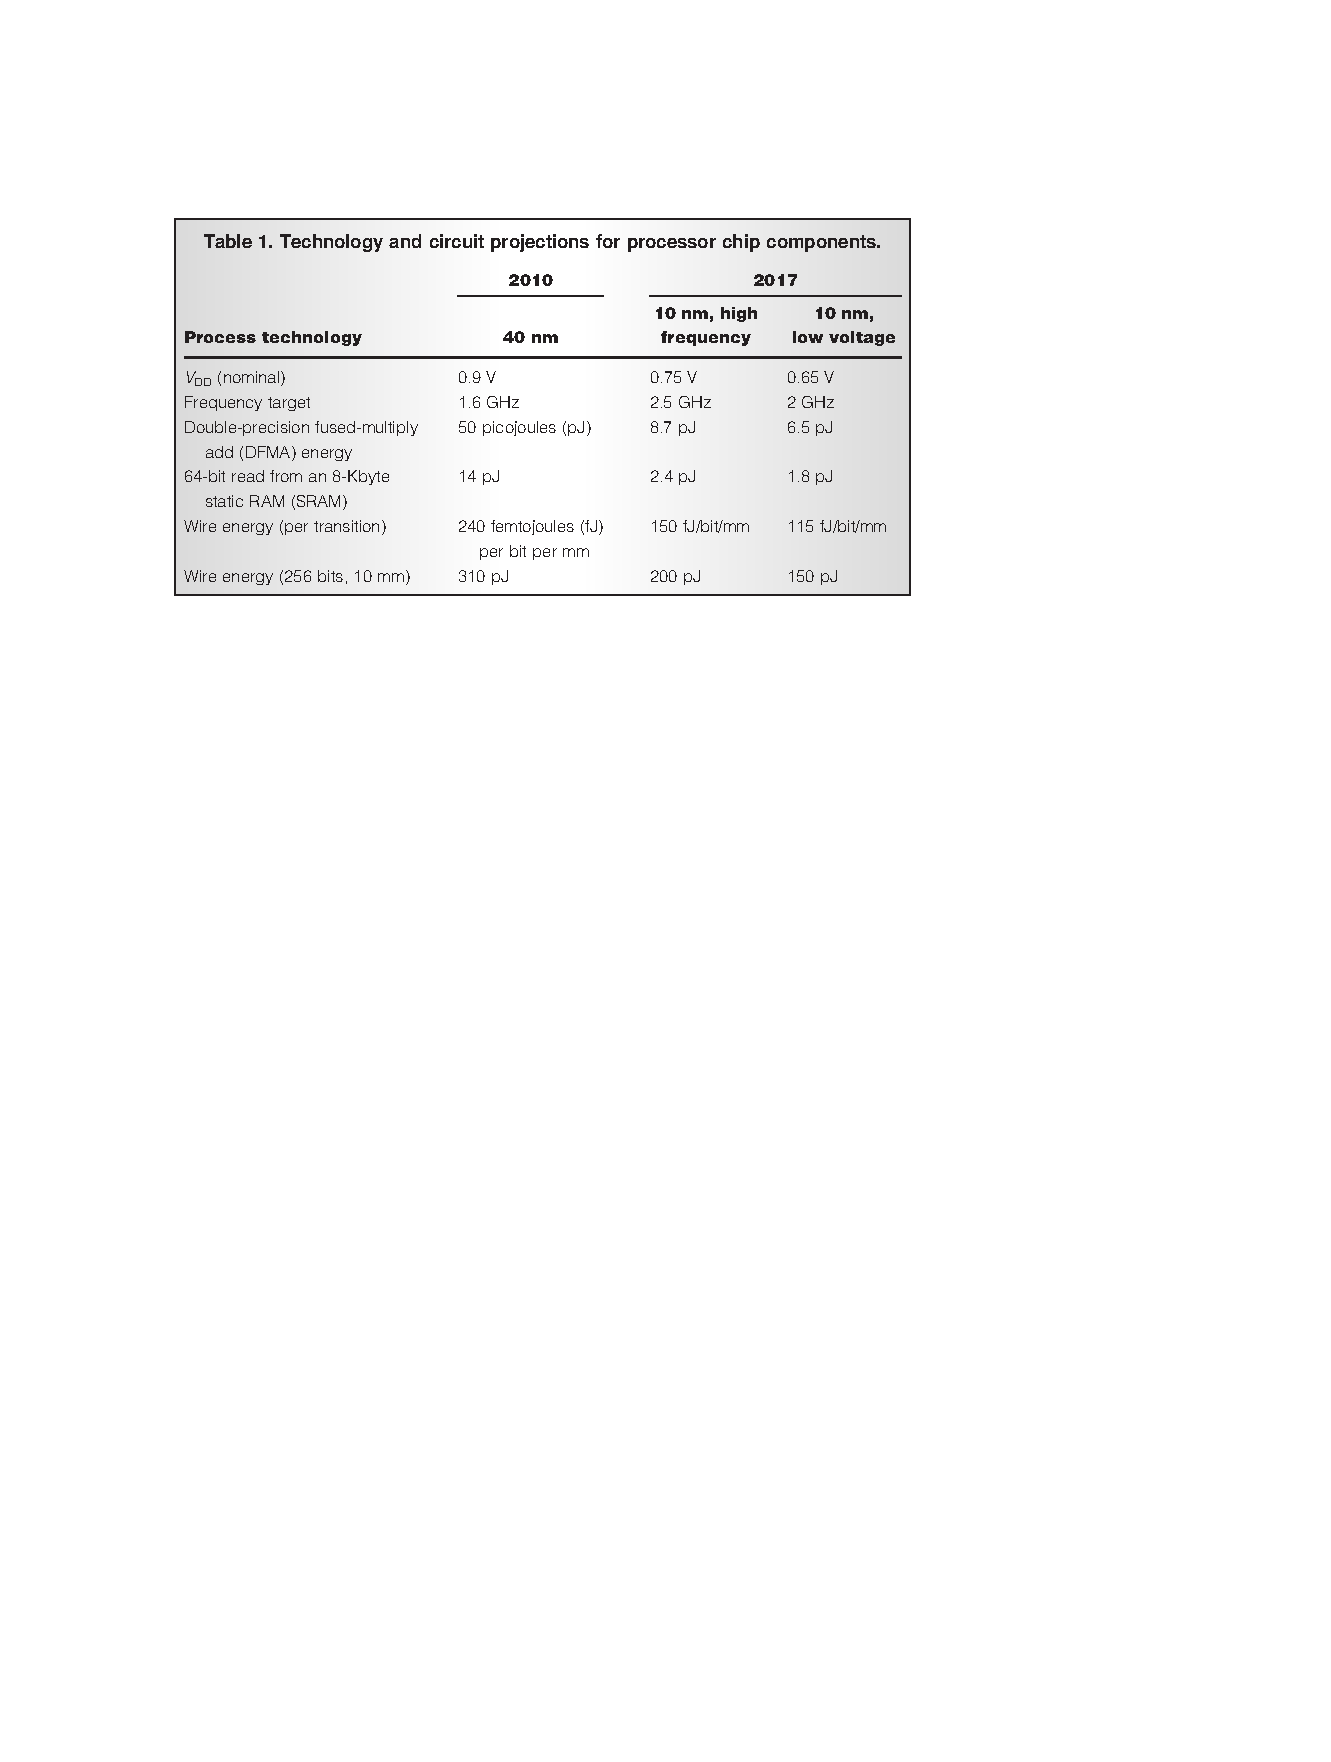
\includegraphics[width=0.95\textwidth]{figures/L13/KecklerEfficiencyTable.pdf}
    \caption{Estimates of energy usage for fused multiply-add operation, accessing data, and moving data on typical processor from 2010 and prediction for processor in 2017. Table source: \cite{keckler2011gpus}.}
    \label{processorEnergy.fig}
\end{figure}

Figure \ref{processorEnergy.fig} illustrates why data movement is such a significant issue for modern processors. The energy dissipated when moving data from RAM to processor depends on distance moved and is considerably larger than the energy expended to perform a fused-multiply-add operation (FMADD). Even if the data moves only 10mm between memory and processor the energy dissipated in the wire during the move exceeds the energy dissipated during the FMADD. 

The HPCG benchmark exposes the quandry of modern computing because it requires a very small number of arithmetic operations  performed for each piece of data moved. Thus performance for HPCG is much lower than LINPACK since the latter performs a very large number of arithmetic operations in dense linear algebra block operations.  Yet somehow the \href{http://top500.org}{top500.org} judges supercomputers by their raw floating point performance not on the strength of their memory systems. Are we building the wrong systems targeting dense linear algebra for huge linear systems that nobody will ever need as measured with the LINPACK benchmark ? The new exascale leadership systems each cost in excess of a half billion USD and they will  inevitably be  judged in part by their LINPACK performance. Digest that for a moment.


\section{Less is Moore}
% https://computing.ornl.gov/workshops/SMC13/presentations/3-SMC_0913_Dally.pdf

In the last section we observed that reading data from system memory consumes a picojoule per bit per 10 mm moved over wire. A picojoule is $10^{-12}J$, a miniscule fraction of a Joule\footnote{Definition: One joule is the equivalent of one watt of power radiated or dissipated for one second. \href{https://en.wikipedia.org/wiki/Joule}{Example from wiki}: ``\emph{The energy required to lift a medium-sized tomato up 1 metre (3 ft 3 in) (assume the tomato has a mass of approximately 100 grams (3.5 oz)).}''}  However, a large scale system running at full capacity will move vast amounts of data. The energy used to move data and  to perform calculations all adds up. For instance, the Summit supercomputer at Oak Ridge National Lab \href{https://www.olcf.ornl.gov/summit/}{consumes up to 13MW}(mega-Watts) of power. For reference 1MW can power approximately 650 homes in the US (see \href{https://m.boiseweekly.com/boise/megawhat/Content?oid=3433953}{for a discussion}).
 
 The power consumption of a large scale computing system has four important ramifications: 
 \begin{enumerate}
     \item {\bf Cost}:  1MW-year of power costs approximately $\$1,000,000$ per year (estimate obtained from this \href{https://www.aqua-calc.com/calculate/electricity-cost}{web-site}.
     \item {\bf Environmental impact}: the power for a supercomputer must be supplied on a continuous and reliable basis. Renewable resources may be an option, but might not meet stringent quality and reliability requirements.
     \item {\bf Power supply}: the DOE leadership facilities are typically collocated with power stations. The maximum reliable load of the power station dictates the power budget for the supercomputer.
     \item {\bf Cooling}: the bi-product of computing is heat, lots of heat. The excess heat needs to be removed requiring considerable cooling systems. Some facilities use excess heat for other purposes.
 \end{enumerate}
The 
\href{https://www.top500.org/green500/lists/2019/06/}{Green Top 500 Supercomputer list} was established to address the issue of improving environmentally sensitive computing. Systems on the Green Top500 list are ranked by metrics like GFLOPS/Watt, i.e. by their computational efficiency. 

According to \href{https://www.top500.org/green500/about/}{the Green Top500 website} 

``\emph{Historically, the Green500 started back in April 2005 – after a keynote talk by Dr. Wu-chun Feng\footnote{Of note, Dr. Feng is currently a Professor of Computer Science at VT !} at the IEEE IPDPS Workshop on High-Performance, Power-Aware Computing.}'' 

%% dominant and emerging architectures
%% exascale roadmap ?

% green top500
% CPU v. GPU
% clock frequency versus core count

\section{HPC programming models}

In the following lectures we will describe the predominant programming models used for developing software for parallel processors and for systems with multiple processors. The main approaches are as follows

\begin{itemize}
    \item {\bf OpenMP}: stands for the Open Multi-Processing standard. It enables a programmer to write code that can fork multiple threads to handle several tasks at the same time on multi-core processors. The OpenMP API consists of functions to manage the number of threads that are forked, to report wall clock time, and to find a thread number. Preprocessor compiler directives (typically starting with \texttt{\#pragma omp}) are used to create parallel regions in code where commands are executed by multiple threads. 
    
    OpenMP is often used to make an existing code run in parallel by light annotation. OpenMP is predicated on all threads having access to shared memory and this limits it typically to running on laptops, desktops, single compute nodes, and recently graphics processing units. Results from using OpenMP can be mixed with variable performance gains depending on the specific problem, quality of implementation, and threading capability of the target processor(s). We will explore the OpenMP philosophy, API, and programming directives in lectures \ref{OpenMPIntro.chap} and \ref{OpenMPadvanced.chap}. 
    
    You will be able to develop and test OpenMP based codes on your laptop using your VirtualBox after which you can deploy it to a \emph{single} compute node on the Advanced Research Computing clusters.
    
    \item{\bf MPI}: stands for the Message Passing Interface. It enables a programmer to write a program that is executed in multiple instances (called processes) at the same time. 
    
    There is no requirement that MPI processes must execute on the same computer. If computers on planet earth and out in space on Mars were networked together then the MPI program could run on both at the same time. The important aspect of an MPI program is that every process executing the program can communicate by passing messages to other instance of the MPI program processes. 
    
    In our hypothetical case a message sent from earth to Mars would take about 13 minutes according to the  \href{http://blogs.esa.int/mex/2012/08/05/time-delay-between-mars-and-earth/}{European Space Agency}. In fact the minimum time it takes to send a message is so fundamental to distributed computing models (as enabled by MPI) that it has a name: latency. Every distributed system has a range of latencies depending on the topology of the network connecting the compute nodes, the type of connections (wire or fibre optic cables), the time lost when messages pass through layers of the operating system, and so on. Usually latency is on the order of milliseconds, with the earth-Mars latency being atypical.
    
    Just like programming in OpenMP, your mileage may vary when using MPI. It is conceptually a little harder to understand what exactly happens when an MPI program executes. However, it is possible to create parallel codes using MPI that scale relatively efficiently up to a million MPI processes running on the largest CPU based supercomputers \cite{balaji2009mpi}.  We will explore the MPI philosophy, API, and programming directives in lectures \ref{MPIIntro.chap},\ref{MPIViz.chap}, \ref{MPICollectives.chap},  and \ref{MPIPerformance.chap}. 
    
    You will be able to develop and test MPI codes on your laptop using your VirtualBox after which you can deploy it to \emph{multiple} compute node on the Advanced Research Computing clusters.
    
    \item {\bf CUDA}: stands for Compute Unified Device Architecture.  It consists of an API and extensions to C. The API enables a programmer to migrate data to and from a GPU from a host computer and to queue up tasks to run on the GPU. The C extensions in CUDA are used by programmers to write so called ``kernels'' that are executed by multiple threads on a GPU. 
    
    The off-load model of GPU computing obliges the programmer to be aware that the CPU and GPU maintain separate physical memory spaces. Data needs to be copied between these spaces and this incurs latency penalties for GPU tasks. Experience CUDA programmers will try to minimize the amount of data that gets copied between the host computer (simply referred to as the ``host'') and the attached GPU (also called the ``device''). A typical model is to set up a problem on the host, copy data over to the device, then do as much work as possible on the device before copying the result back to the host. 
    
    It is important to note that CUDA is a proprietary API and programming language provided by NVIDIA and is typically restricted to being used on their GPUs. This arrangement is sometimes referred to as a vendor locked ecosystem. Developing software under such an arrangement means that the resulting code depends on continued support of a commercial company to be usable. This obviously entails some risk.
    
     Just like programming in OpenMP and MPI, your mileage may vary when using CUDA. It is conceptually quite a bit harder to understand what exactly happens when an CUDA program executes on a GPU. However, carefully crafted CUDA GPU code can achieve a high percentage of peak performance.
     
     You may be able to use your laptop or desktop to develop and test CUDA code if it has an NVIDIA GPU. However it may not be possible to do this through the VirtualBox as you may not be able to access the GPU through the virtualization layer.  You will be able to develop and test CUDA codes on a GPU equipped compute node on the Cascades Advanced Research Computing cluster.
     
\end{itemize}

There are additional GPU programming models that we will introduce but not discuss directly.

\begin{itemize}
    \item {AMD HIP}: stands for \href{https://gpuopen.com/compute-product/hip-convert-cuda-to-portable-c-code/}{Heterogeneous-Compute Interface for Portability}. It enables a programmer to write code that can execute on AMD GPUs or on NVIDIA GPUs (via translation). It lacks some CUDA functionality that relies on hardware specific features exclusive to NVIDIA GPUs, but otherwise the API calls are very similar except \texttt{cuda} is replaced with \texttt{hip} in function names.
    
    \item {OpenCL}: stands for \href{https://en.wikipedia.org/wiki/OpenCL}{Open Computing Language}. OpenCL is an open standard proposed by the \href{https://www.khronos.org/opencl/}{Khronos Group} and brings a CUDA inspired programming model to  CPUs, GPUs, field programmable gate arrays (FPGAs), and even embedded processors. The start up cost for programmers starting with vanilla OpenCL is higher than CUDA. The extra complexity of using OpenCL boils down to the broad range of hardware processors and OpenCL implementations that have to be accommodated when starting an OpenCL computation. One notable feature of using OpenCL is that unlike CUDA it does not require a special compiler as it is entirely library based.
    
    \item {SyCL}: \href{https://www.khronos.org/sycl/}{single source hetergeneous programming for OpenCL} brings a C++ front end to OpenCL.
    
    \item {OpenACC}: stands for \href{https://en.wikipedia.org/wiki/OpenACC}{Open Accelerator}. It is similar in spirit to OpenMP but designed to target primarily offload computing with GPUs. 
\end{itemize}

\section{That's all ``nice'' but what about the cloud ?}

Where HPC goes, the \faCloud{} follows. The mechanics and traditions of Linux terminal based computing that originated in large part with HPC translate immediately to the cloud. The ``cloud'' is after all largely just a collection of compute and storage nodes likely running Linux. Cloud computing instances come equipped with every available CPU and some include GPU(s). 

The heavy computational demands of training deep neural networks has resulted in the major cloud providers making compute instances available with heavyweight GPUs, in particular the NVIDIA Volta V100 GPU is a popular configuration option because of its built in specialized tensor cores.

The price of an instance depends on the capability of the CPU/GPU. To maximize the return on investment you really should use every CPU/GPU core available and that obliges you to use and/or write computer codes that are enabled for parallel computing !


\section{Definitions}

Here are some acronyms and phrases that you will hear repeatedly in the rest of the semester.

\begin{itemize}
    \item \href{https://en.wikipedia.org/wiki/SIMD}{Single Instruction Multiple Data} (SIMD): one instruction stream (i.e. set of code instructions) being used to simultaneously process multiple sets of data in lockstep.
    \item \href{https://en.wikipedia.org/wiki/SPMD}{Single Program Multiple Data} (SPMD): one program executed multiple times on separate data sets, not forced to process in lockstep. MPI programs fall loosely into this category.
    \item \href{https://en.wikipedia.org/wiki/Flynn's_taxonomy}{Flynn's taxonomy}: a classification scheme for different parallel programming models.
    \item \href{https://en.wikipedia.org/wiki/Directive_(programming)}{Compiler directive} (or pragma): an instruction in source code that a compiler may elect to modify the way the program is compiled.
    \item \href{https://en.wikipedia.org/wiki/Graphics_processing_unit}{Graphics Processing Unit} (GPU, device, or accelerator): a quasi-autonomous computer attached to a host computer. 
    \item \href{https://en.wikipedia.org/wiki/Vector_processor}{Vector processing unit} (or SIMD unit): hardware capable of executing a SIMD program. 
    \item Vector lane: a single floating point unit in a vector processing unit.
    \item Thread: a single stream of program instructions.
    \item Warp (or wavefront): a group of threads that are processed in SIMD fashion, i.e. in lockstep, concurrently on a GPU SIMD unit. 
    \item Single Instruction Multiple Threads (SIMT): NVIDIA  refers to their specific GPU version of SIMD as SIMT, distinct from SIMD, because each lane in the vector processing units of their GPU cores  can execute either an instruction or a non-operation (NOP).
    \item \href{https://en.wikipedia.org/wiki/Network_interface_controller}{Network Interface Controller} (NIC): hardware that sits between the CPU and the external network. 
    \item \href{https://en.wikipedia.org/wiki/Processor_register}{CPU Register}: fast memory store collocated with processor core.
    
\end{itemize}